\subsubsection{Company}
Meanwhile companies can also access the site to gain access to students. For example a recruiter from Netcraft, Sally, wishes to sign up in order to find students for placements.
  \paragraph{Sign up:}
    If Netcraft had not yet registered as a company, then the Sally must sign up on Netcrafts behalf, which is very similar to the student signup page.
    Since Netcraft already exists then Sally must request that another admininistrator adds her by signing in and clicking on the new administrator button.

  \paragraph{Contacts:}
    Sally decides that she wishes to be contacted by students regarding job oppourtunities so adds her details to the company contacts in the top right hand corner. This very nicely comes up with an in place form for Sally to fill out.
    Sally is pleased when her contact card appears at the top but just incase she wanted to move herself below anyone else she notices the useful tooltip that tells her contact cards are draggable.

    \begin{figure}[H]\centering
    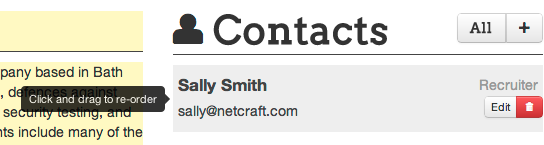
\includegraphics[scale=0.5]{images/user_experiences/company/netcraft_company_contact_tooltip}
    \caption{Tooltip for company contacts}
    \end{figure}
    Students viewing this page can then email any of the contacts since they must disclose their email addresses.

    We have also added tooltips to the all contacts page incase a company decides to create a contact from there. They will then know that any of these contact cards are draggable.

  \paragraph{Events and Placements:}
    Sally decides that it might be a good idea to post that Netcraft is offering six month industrial placements and so clicks on the new placement button. 
    She receives important notices from the departments she's registered to that she reads and makes note of and then procedes to create the placement.
    Similarly Sally can do the exact same thing with events.

    Sally then decided to look at an event that Netcraft is already advertising, as the event is coming up very soon she has the option to email the students more useful information, like how to get to Netcraft from the train station.
    This email will only be sent to receipients that are actually attending the event.
  
  \paragraph{Students:}
    After creating placements and events Sally decides she wants to browse students to find exceptional candidates she can contact herself. She clicks on students on the navigation bar and is greeted by a list of students. Note that any students who have decided to black Netcraft will never appear in this list, nor will deactivated students.
    Since she knows Netcraft will be recruiting for Perl developers, she specifically types Perl into the skills filter
    and filters the list down to the students who have it as a skill.
    %TODO print screen
    She can then browse their profiles, which is a reduced version of the student view lacking the events and placement partial views since they are not relevant to her.

    \begin{figure}[H]\centering
    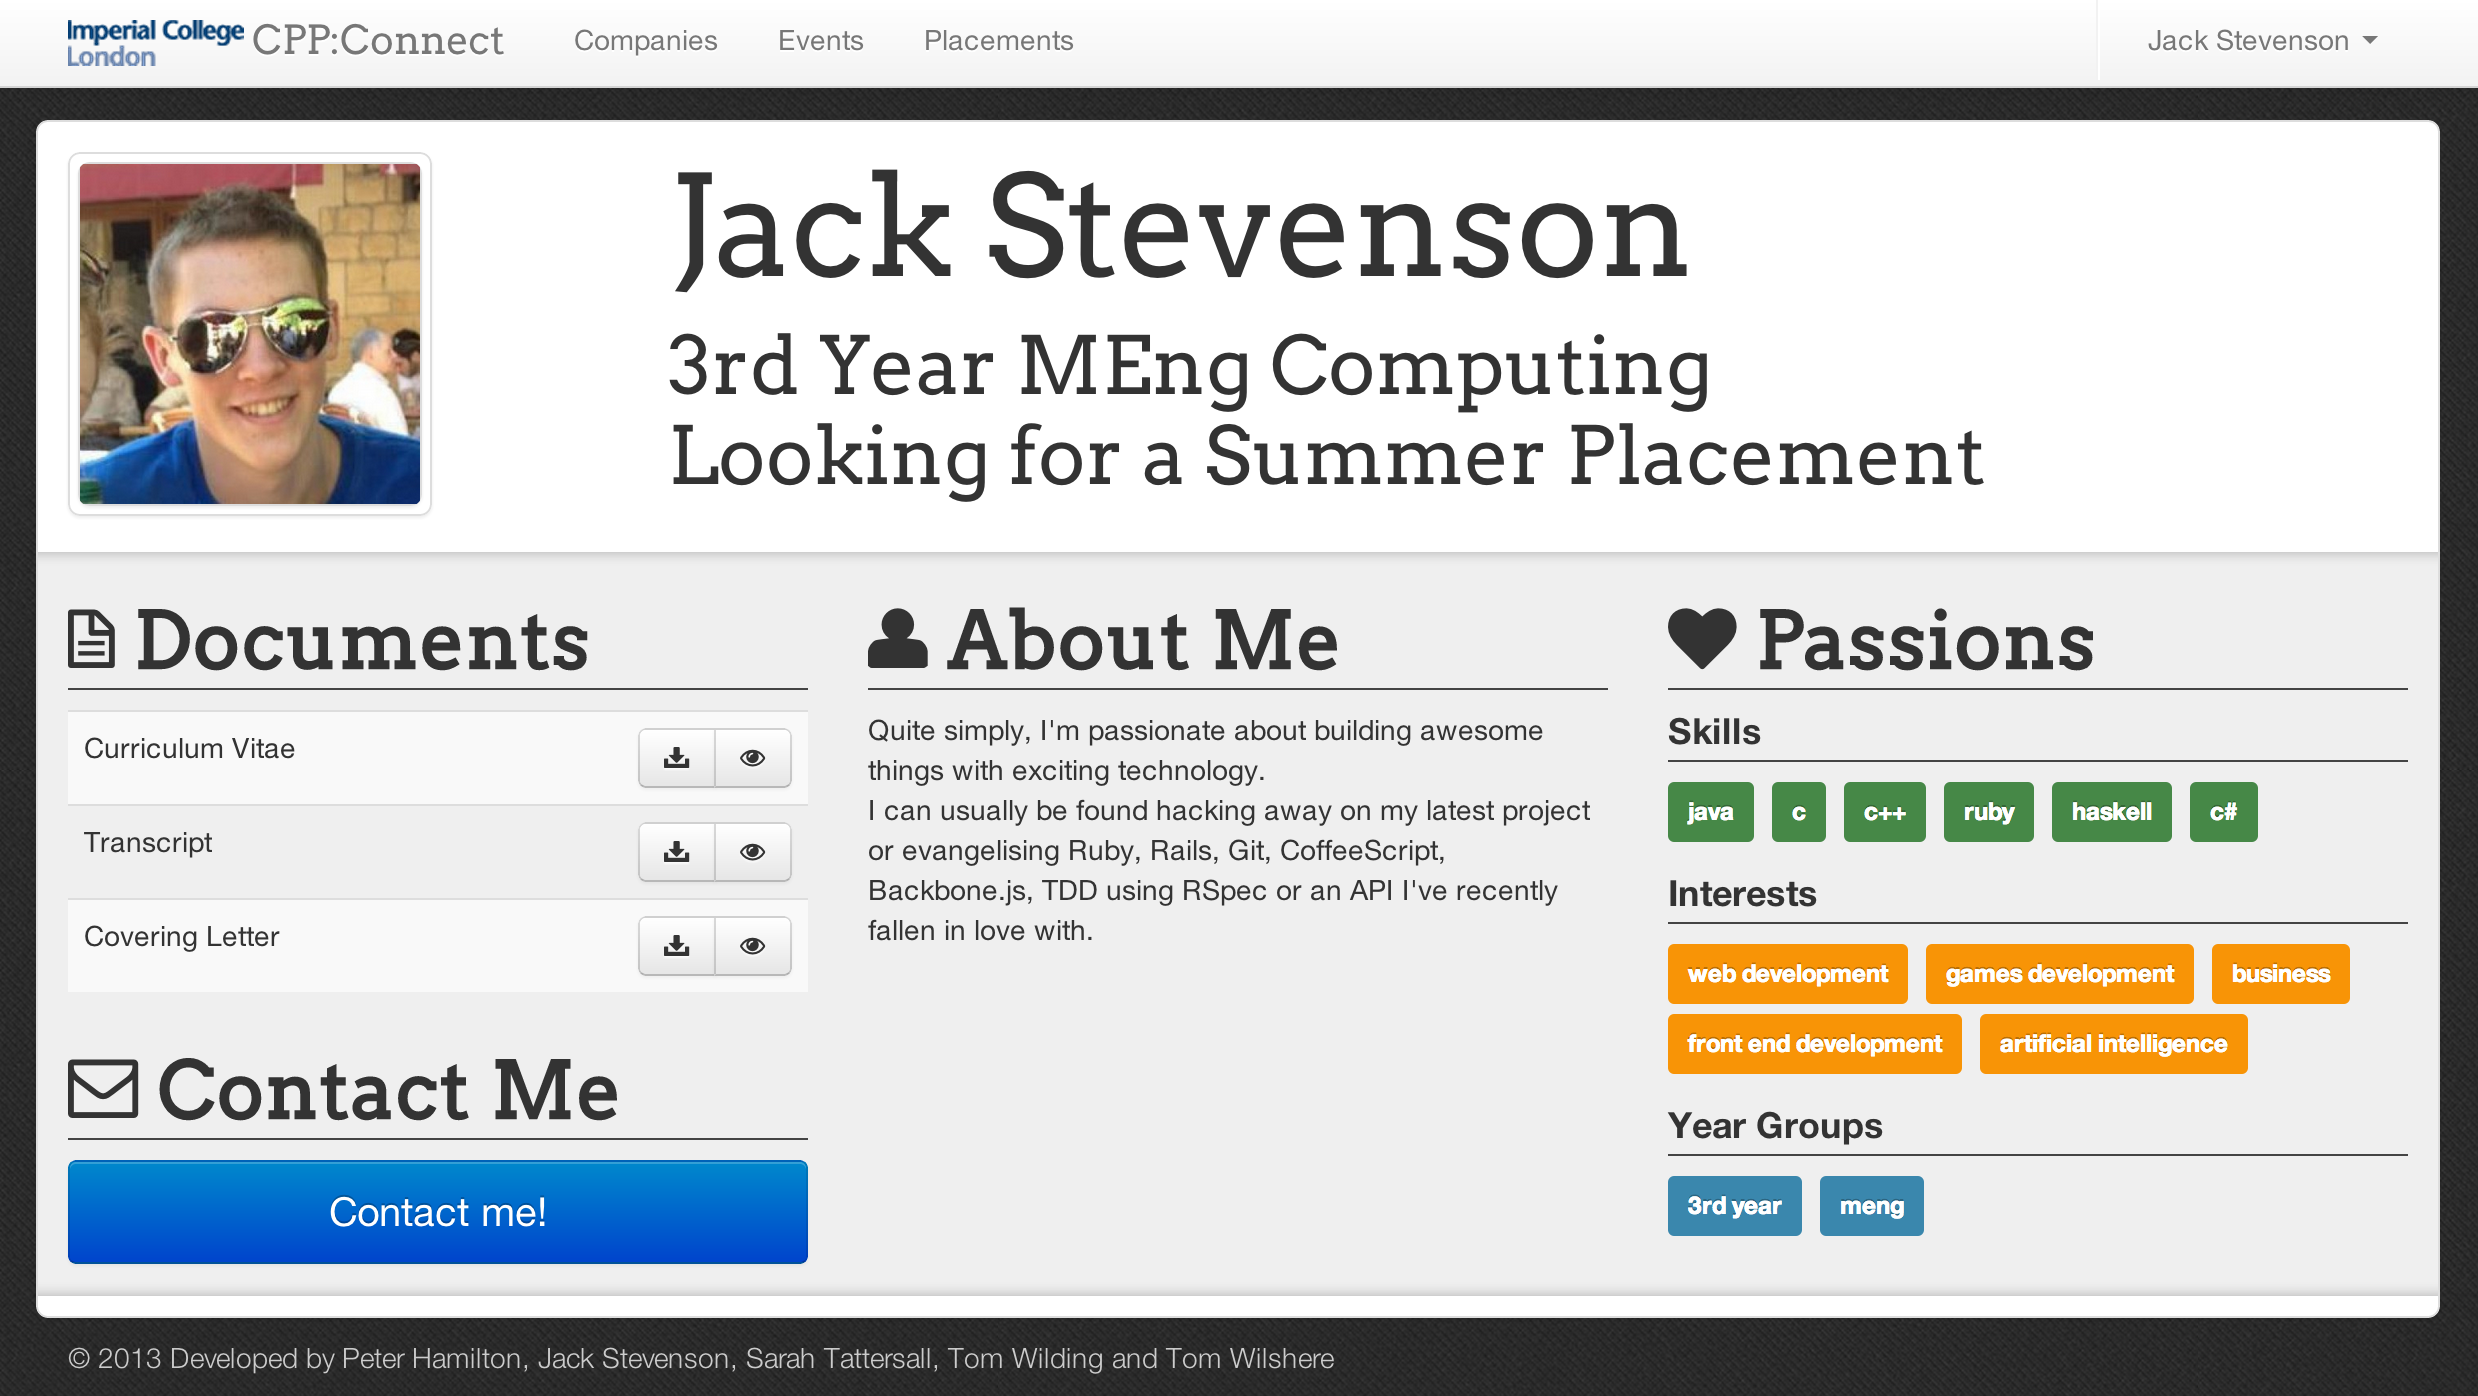
\includegraphics[scale=0.3]{images/user_experiences/company/jack_profile}
    \caption{Company view of student profile}
    \end{figure}

    Liking what she see's Sally can then choose to download Jack's CV to her computer or view it online with the preview icon button. 

    %TODO CLICK ON MAIL ICON
    Finally after reading Jacks CV Sally then chooses to invite Jack to interview, by clicking on the contact student button. She then sends an email from her account to his address which he can reply to if he wants. 

  \paragraph{Emails:}
    Being a member of the Corporate Partnership Program also entitles Netcraft to be able to contact a departments students via email. Sally can create emails to inform students of exciting scholarships Netcraft are offering, or news about the company.

    Once she has written and sent her emails (including those sent previously) she must wait for them to be approved by an admin.

    We have chosen for emails to be approved by an admin to avoid companies being able to spam students. We hope that the need for admin approval encourages them to write detailed informative emails that are of an appropriate content for students. If it is not deemed applicable enough the admin can send the email back to the company for modifying with the reason, or reject it all together.

    %%%%%%%%%%%%%%%%%%%%%%%%%%%% TODO %%%%%%%%%%%%%%%%%%%%%%%%%%%%%
    % * Companies requesting permissions for students, perhaps Sally wants Maths students?
    % * Print screens
    % * Describe a little more about the emails
    %%%%%%%%%%%%%%%%%%%%%%%%%%%%%%%%%%%%%%%%%%%%%%%%%%%%%%%%%%%%%%%
